\newpage

\section{Messergebnisse}

\begin{table}
  \centering
  \caption{Gemessene Werte bei der Wheatstoneschen Brücke}
  \label{tab:Wheatstone}
  \begin{tabular}{ c c c c c }
    \toprule
      & & Messung 1 & Messung 2 & Messung 3 \\
    \midrule
    Wert 10 & \multicolumn{1}{c|}{$\su{R_2}$  in  $\su{\Omega} $ } & 1000 & 664 & 332 \\
            & \multicolumn{1}{c|}{$\su{R_3}$  in  $\su{\Omega} $ } & 196 & 268 & 422  \\
            & \multicolumn{1}{c|}{$\su{R_4}$  in  $\su{\Omega} $ } & 804 & 732 & 578  \\
    \midrule
    Wert 12 & \multicolumn{1}{c|}{$\su{R_2}$  in  $\su{\Omega} $ } & 1000 & 664 & 332 \\
            & \multicolumn{1}{c|}{$\su{R_3}$  in  $\su{\Omega} $ } & 284 & 373 & 543  \\
            & \multicolumn{1}{c|}{$\su{R_4}$  in  $\su{\Omega} $ } & 716 & 627 & 457  \\
    \bottomrule
  \end{tabular}
\end{table}

\begin{table}
  \centering
  \caption{Gemessene Werte für die Kapazitätsmessbrücke ohne Wiederstände}
  \label{tab:Kapazitätohne}
  \begin{tabular}{ c c c c c }
    \toprule
    & & Messung 1 & Messung 2 & Messung 3 \\
    \midrule
    Wert 3 & \multicolumn{1}{c|}{$\su{C_2}$  in  $\su{nF}    $}  & 450 & 399 & 597  \\
           & \multicolumn{1}{c|}{$\su{R_3}$  in  $\su{\Omega}$}  & 519 & 490 & 590  \\
           & \multicolumn{1}{c|}{$\su{R_4}$  in  $\su{\Omega}$}  & 481 & 510 & 410  \\
    \midrule
    Wert 1 & \multicolumn{1}{c|}{$\su{C_2}$  in  $\su{nF}    $}  & 450 & 399 & 597 \\
           & \multicolumn{1}{c|}{$\su{R_3}$  in  $\su{\Omega}$}  & 407 & 380 & 478 \\
           & \multicolumn{1}{c|}{$\su{R_4}$  in  $\su{\Omega}$}  & 593 & 520 & 522 \\
    \bottomrule
  \end{tabular}
\end{table}


\begin{table}
  \centering
  \caption{Gemessene Werte für die Kapazitätsmessbrücke mit Wiederständen}
  \label{tab:Kapazitätmit}
  \begin{tabular}{ c c c c c}
    \toprule
    & & Messung 1 & Messung 2 & Messung 3 \\
    \midrule
    Wert 8 & \multicolumn{1}{c|}{$\su{C_2}$  in  $\su{nF}     $ } & 450 & 399 & 597 \\
           & \multicolumn{1}{c|}{$\su{R_2}$  in  $\su{\Omega} $ } & 371 & 418 & 278 \\
           & \multicolumn{1}{c|}{$\su{R_3}$  in  $\su{\Omega} $ } & 606 & 578 & 673 \\
           & \multicolumn{1}{c|}{$\su{R_4}$  in  $\su{\Omega} $ } & 394 & 422 & 327 \\
    \midrule
    Wert 9 & \multicolumn{1}{c|}{$\su{C_2}$  in  $\su{nF}     $ } & 450 & 399 & 597 \\
           & \multicolumn{1}{c|}{$\su{R_2}$  in  $\su{\Omega} $ } & 466 & 524 & 352 \\
           & \multicolumn{1}{c|}{$\su{R_3}$  in  $\su{\Omega} $ } & 511 & 481 & 581 \\
           & \multicolumn{1}{c|}{$\su{R_4}$  in  $\su{\Omega} $ } & 489 & 519 & 419 \\
    \bottomrule
  \end{tabular}
\end{table}


\begin{table}
  \centering
  \caption{Gemessene Werte für die Induktivitätmessbrücke}
  \label{tab:Induktivitätsmessbrücke}
  \begin{tabular}{ c c c c c}
    \toprule
    & & Messung 1 & Messung 2 & Messung 3 \\
    \midrule
    Wert 10 & \multicolumn{1}{c|}{$\su{L_2}$  in  $\su{mH}     $ } & 14.6 & 20.1 & 27.5 \\
            & \multicolumn{1}{c|}{$\su{R_2}$  in  $\su{\Omega} $ } & 45  & 57  & 85  \\
            & \multicolumn{1}{c|}{$\su{R_3}$  in  $\su{\Omega} $ } & 907 & 875 & 837 \\
            & \multicolumn{1}{c|}{$\su{R_4}$  in  $\su{\Omega} $ } & 83  & 125 & 163 \\
    \midrule
    Wert 18 & \multicolumn{1}{c|}{$\su{L_2}$  in  $\su{mH}     $ } & 14.6 & 20.1 & 27.5 \\
            & \multicolumn{1}{c|}{$\su{R_2}$  in  $\su{\Omega} $ } & 108 & 143 & 197 \\
            & \multicolumn{1}{c|}{$\su{R_3}$  in  $\su{\Omega} $ } & 775 & 715 & 648 \\
            & \multicolumn{1}{c|}{$\su{R_4}$  in  $\su{\Omega} $ } & 225 & 285 & 352 \\
    \bottomrule
  \end{tabular}
\end{table}


\begin{table}
  \centering
  \caption{Gemessene Werte für R-L-Glieder mit der Maxwell-Brücke}
  \label{tab:Maxwell}
  \begin{tabular}{ c c c c c }
    \toprule
    & & Messung 1 & Messung 2 & Messung 3 \\
    \midrule
    Wert 10 & \multicolumn{1}{c|}{$\su{R_2}$  in  $\su{\Omega} $ } & 100 & 664 & 332 \\
            & \multicolumn{1}{c|}{$\su{R_3}$  in  $\su{\Omega} $ } & 347 & 523 & 1036 \\
            & \multicolumn{1}{c|}{$\su{R_4}$  in  $\su{\Omega} $ } & 829 & 829 & 829 \\
    \midrule
    Wert 18 & \multicolumn{1}{c|}{$\su{R_2}$  in  $\su{\Omega} $ } & 100 & 664 & 332 \\
            & \multicolumn{1}{c|}{$\su{R_3}$  in  $\su{\Omega} $ } & 128 & 193 & 382 \\
            & \multicolumn{1}{c|}{$\su{R_4}$  in  $\su{\Omega} $ } & 347 & 349 & 348 \\
    \bottomrule
  \end{tabular}
\end{table}

\begin{table}
  \centering
  \caption{Gemessene Werte bei der Wien-Robinson-Brücke}
  \label{tab:MessungE}
  \begin{tabular}{ c c c}
    \toprule
    $\su{\nu}$ in $\su{\frac{1}{s}}$ & $\su{U\ua{Br}}$ in V & $\su{U\ua{Sp}}$ in V \\
    \midrule
    20    & 2.480 & 2.700 \\
    100   & 1.960 & 2.550 \\
    200   & 1.000 & 2.200 \\
    270   & 0.524 & 2.000 \\
    320   & 0.260 & 1.800 \\
    340   & 0.172 & 1.800 \\
    360   & 0.078 & 1.700 \\
    370   & 0.044 & 1.700 \\
    390   & 0.053 & 1.650 \\
    395   & 0.084 & 1.650 \\
    400   & 0.094 & 1.650 \\
    405   & 0.136 & 1.650 \\
    410   & 0.140 & 1.600 \\
    415   & 0.166 & 1.600 \\
    420   & 0.184 & 1.600 \\
    430   & 0.210 & 1.600 \\
    440   & 0.254 & 1.550 \\
    469   & 0.328 & 1.500 \\
    480   & 0.384 & 1.450 \\
    500   & 0.468 & 1.400 \\
    550   & 0.590 & 1.250 \\
    600   & 0.740 & 1.200 \\
    700   & 1.020 & 1.100 \\
    800   & 1.150 & 0.950 \\
    1000  & 1.450 & 0.750 \\
    1200  & 1.660 & 0.680 \\
    1500  & 1.860 & 0.540 \\
    2000  & 2.000 & 0.410 \\
    3000  & 2.140 & 0.285 \\
    5000  & 2.180 & 0.175 \\
    10000 & 2.040 & 0.090 \\
    20000 & 1.660 & 0.060 \\
    30000 & 1.180 & 0.055 \\
    \bottomrule
  \end{tabular}
\end{table}

\section{Auswertung}

\subsection{Wheatstonesche Brückenschaltung}
Mit den gemessenen Werte aus Tabelle \ref{tab:Wheatstone} und der Formel \eqref{eqn:Wheatstone}
lassen sich nun die gesuchten
Widerstände berechnen. Dabei ergeben sich folgende Werte:

\begin{align}
  \su{R\ua{x,10}} &= (243.1 \pm 0.4) \, \su{\Omega} \\
  \su{R\ua{x,12}} &= (395.4 \pm 0.7) \, \su{\Omega}
\end{align}

\subsection{Kapazitätsmessbrücke}

Mit den Werten aus Tabelle \ref{tab:Kapazitätohne} für die Kapazitätsmessbrücke
ohne zwischengeschaltete Widerstände und der Formel \eqref{KapazitätsmessbrückeLx}
ergeben sich für die gesuchten Kapazitäten die folgenden Werte:

\begin{align}
  \su{C\ua{x,1}} &= (652.9 \pm 1.4) \, \su{nF} \\
  \su{C\ua{x,3}} &= (415.7 \pm 0.7) \, \su{nF}
\end{align}

Mit den Werten aus Tabelle \ref{tab:Kapazitätmit} für die Kapazitätsmessbrücke
mit Widerständen und den Formen \eqref{KapazitätsmessbrückeRx} und \eqref{KapazitätsmessbrückeLx}
lassen sich ebenfalls die gesuchten Werte der R-C-Glieder bestimmen:

\begin{align}
  \su{R\ua{x,8}} &= (571.8 \pm 0.6) \, \su{\Omega} \\
  \su{C\ua{x,8}} &= (291.3 \pm 0.7) \, \su{nF}
\end{align}

\begin{align}
  \su{R\ua{x,9}} &= (487.6 \pm 0.3) \, \su{\Omega} \\
  \su{C\ua{x,9}} &= (430.0 \pm 0.6) \, \su{nF}
\end{align}

\subsection{Induktivitätsmessbrücke}

Mit den Formeln \eqref{InduktivitätmessbrückeRx} und \eqref{InduktivitätmessbrückeLx}
und den Werten aus der Tabelle \ref{tab:Induktivitätsmessbrücke}
ergeben sich für die gesuchten R-L-Glieder folgende Werte:

\begin{align}
  \su{R\ua{x,16}} &= (442 \pm 27) \, \su{\Omega} \\
  \su{L\ua{x,16}} &= (147 \pm 6) \, \su{mH}
\end{align}

\begin{align}
  \su{R\ua{x,18}} &= (364 \pm 4) \, \su{\Omega}  \\
  \su{L\ua{x,18}} &= (50.5 \pm 0.1) \, \su{mH}
\end{align}

\subsection{Maxwell-Brücke}
Die gleichen R-L-Glieder wie bei der Induktivitätsmessbrücke wurden nochmal mithilfe
der Maxwell-Brücke gemessen, bei der ein Kondensator mit der Kapazität $\su{C_4} = 399 \, nF$
verwendet wurde. Mit den Werte aus der Tabelle \ref{tab:Maxwell}
sowie den Formeln \eqref{eqn:Maxwell_Rx} und \eqref{eqn:Maxwell_Lx} ergeben sich
für die beiden R-L-Glieder somit folgende Werte:

\begin{align}
  \su{R\ua{x,16}} &= (417.5 \pm 1.3) \, \su{\Omega} \\
  \su{L\ua{x,16}} &= (138.1 \pm 0.4) \, \su{mH}
\end{align}

\begin{align}
  \su{R\ua{x,18}} &= (366.8 \pm 1.3) \, \su{\Omega}  \\
  \su{L\ua{x,18}} &= (50.94 \pm 0.17) \, \su{mH}
\end{align}

\subsection{Robinson-Wien-Brücke}

Bei der Messung die für Robinson-Wien-Schaltung wurden die folgenden Komponenten
verwendet:

\begin{align}
  \su{C}   &=  (415.7 \pm 0.7) \, \su{nF}  \\
  \su{R'}  &= 332 \, \su{\Omega}          \\
  \su{2R'} &= 664 \, \su{\Omega}         \\
  \su{R}   &= 1000 \, \su{\Omega}
\end{align}

In dieser Messreihe wurde die Frequenzabhängigkeit der Brückenspannung untersucht.
Dazu wird in den Graphen \ref{Plotkomplett} und \ref{Plotgeschnitten}
das Verhältnis der effektiven Brückenspannung $\su{U\ua{Br,eff}}$
zur Speisespannung $\su{U\ua{Sp}}$ gegen $\su{\Omega}$ = $\frac{\su{\nu}}{\su{\nu_0}}$
aufgetragen. Für $\su{U\ua{Br,eff}}$ gilt dabei:

\begin{equation}
  \su{U\ua{Br,eff}} = \frac{\su{U\ua{Br}}}{2\sqrt{2}}.
  \label{eqn:Ubreff}
\end{equation}

Als Frequenz, bei der die Brückenspannung verschwinden sollte, ergibt sich folgender
Wert:

\begin{align}
  \su{\omega_0} &= \frac{1}{\u{RC}} = \frac{1}{1000 \, \su{\Omega} \cdot (415.7 \pm 0.7) \cdot 10^{-9} \, \su{F}} = (2406 \pm 4) \, \su{Hz} \\
  \su{\nu_0}    &= \frac{\su{\omega_0}}{2\pi} = (382.9 \pm 0.6) \, \su{Hz}
\end{align}

\begin{figure}
  \centering
  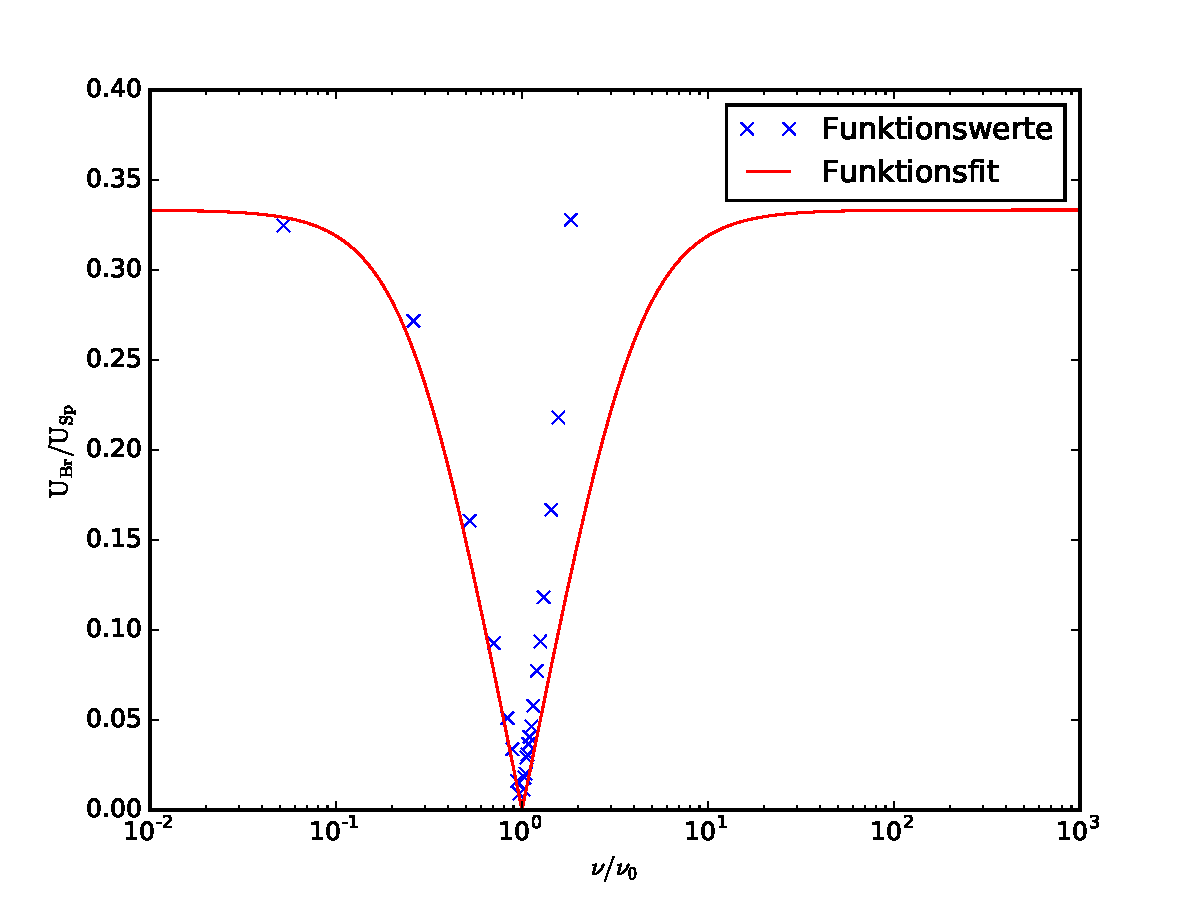
\includegraphics[height = 9.0 cm]{Plot_klein.pdf}
  \caption{Vergleich der Messdaten mit einer Theoriekurve im kleineren Bildintervall}
  \label{Plotgeschnitten}
\end{figure}

\begin{figure}
  \centering
  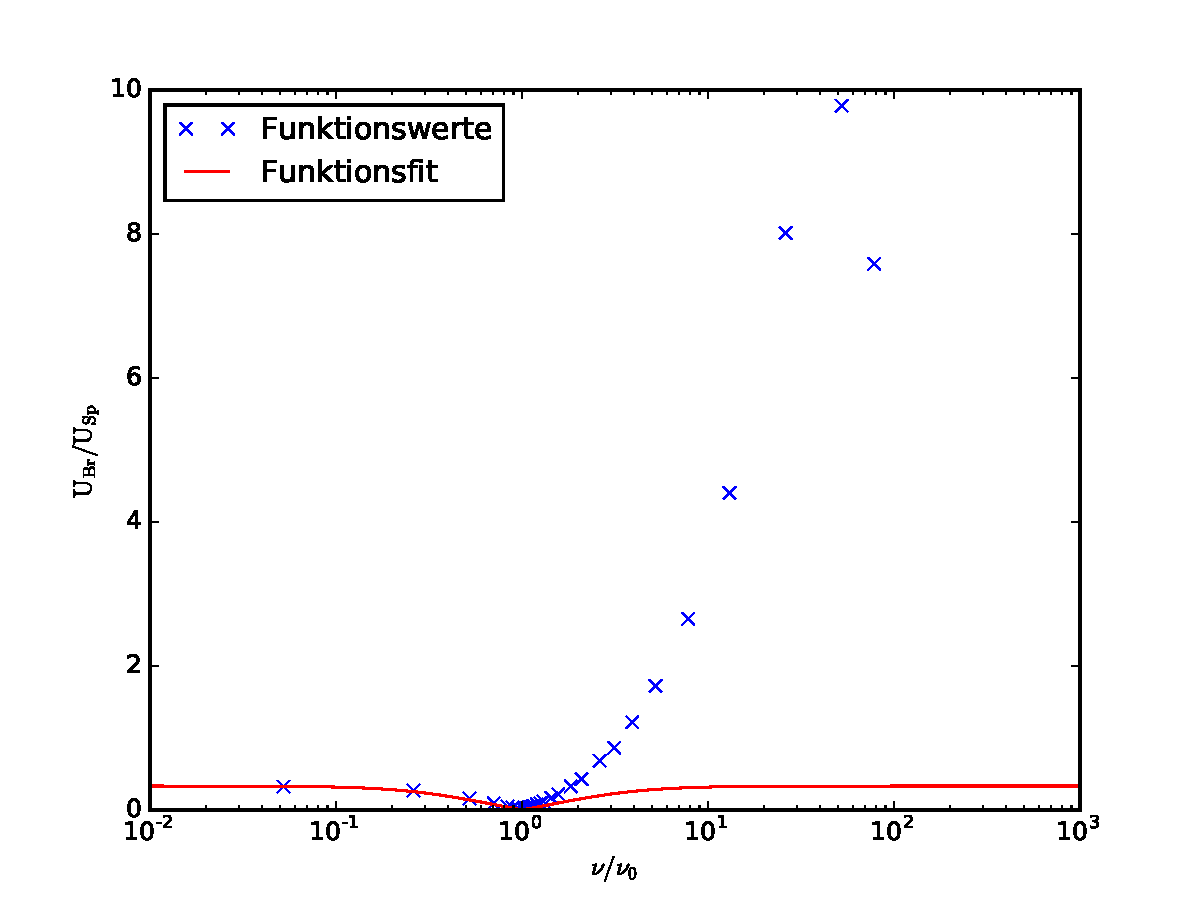
\includegraphics[height = 9.0 cm]{Plot_gross.pdf}
  \caption{Vergleich der Messdaten mit einer Theoriekurve}
  \label{Plotkomplett}
\end{figure}

In dem folgendem Abschnitt wird mit der bereits durch Formel \eqref{eqn:Ubreff}
bestimmten Effektivspannung
weitergerechnet, um den Klirrfaktor zu bestimmen. Zur Vereinfachung der Rechnung
wird dabei genähert, dass die Summe der Oberwellen lediglich von dem Term der
zweiten Oberwelle bestimmt wird.

Mit Formel \eqref{eqn:Klirrfaktor} werden zu Berechnung noch die Werte für $\su{U_2}$ und $\su{U_1}$ bestimmt,
wobei $\su{U_1}$ die 1,65 V von $\su{U\ua{Sp}}$ bei $\su{\nu_0}$ sind. Aus der Formel
\eqref{eqn:Wien-Robinson-Brücke}
und $\su{\Omega}$ = 2 errechnet sich $U\ua{2}$ dann wie folgt:

\begin{align}
  \su{U_2} &= \frac{\su{U\ua{Br,eff}}}{f(2)} \\
           &= 4.269 \cdot 10^{-2} \, \su{V}.
\end{align}

Der Klirrfaktor ergibt sich damit nun aus dem Quotienten von $\su{U_2}$ und
$\su{U_1}$:

\begin{equation}
  \su{k} = \frac{\su{U_2}}{\su{U_1}} = 2.668 \cdot 10^{-2}.
\end{equation}

\newpage


\section{Diskussion}

In dem folgenden Abschnitt soll nun betrachtet werden, inwieweit die verwendeten
Messmethoden zuverlässige Ergebnisse liefern.

Bei allen Messungen ist deutlich erkennbar, dass die Fehler der einzelnen Bauteile
relativ gering ausfallen. Somit lässt sich auf eine systematisch korrekte und
ziemlich genaue Messung schließen.

Ein Vergleich der auftretenden Fehler bei den Messungen 4.3 und 4.4, der
Induktivitätsmessbrücke und der Maxwell-Brücke, zeigt einen deutlichen Unterschied
bei den entstehenden Fehlern. Die Fehler der Maxwell-Brücke fallen deutlich geringer
aus, was vor allem an der Annahme liegen könnte, dass die verwendete
Spule $\su{L_2}$ bei der Induktivitätsmessbrücke keinen Innenwiderstand besitzt,
was in der Messung nicht realisierbar ist.
Zwar wurde auch bei der Maxwell-Brücke der Kondensator als verlustfrei angenommen,
dies lässt sich jedoch weitaus besser realisieren. Dennoch sind die Abweichungen
der gemessenen Werte beider Methoden nicht allzu groß, die Maxwell-Brücke
scheint in dieser Messung lediglich genauer zu sein.

Bei der Bestimmung des Klirrfaktors sieht man, dass die gemessenen Werte besonders
bei Frequenzen oberhalb des Minimums stark von der Theoriekurve abweichen. Da die
Form der Kurve jedoch ähnlich ist, kann man auf einen systematischen Fehler schließen.
Dies ist schon in den Messwerten zu erkennen, in denen die Speisespannung eigentlich
relativ konstant bleiben sollte, jedoch zwischenzeitlich auf ca. 3 $\%$ des
ursprünglichen Wertes absinkt. Somit kann der Klirrfaktor als Beurteilung der
Güte des Sinusgenerators eigenlich nur bedingt verwendet werden. Dennoch ist
der Wert trotz der Messungenauigkeiten ziemlich gering.
